\documentclass[ASNA,twocolumn]{USG}
\usepackage{anyfontsize}
\usepackage{colortbl}
\usepackage{xcolor}
\usepackage{steinmetz}
\usepackage{booktabs}
\usepackage{enumitem}
\usepackage{graphicx}
\graphicspath{{./images/}{../MDPI/figures/}}

\specialissue{Campus-DDoS-SDN: Multi-vector DDoS detection in software-defined campus networks}
\articletype{ORIGINAL ARTICLE}
\subarticletype{Software-defined networking and security}
\received{4 November 2026}
\revised{4 November 2026}
\accepted{4 November 2026}
\journal{Computer Networks}
\volume{0}
\copyyear{2026}
\startpage{1}
\articledoi{10.1002/0000}

\begin{document}

\title{Campus-DDoS-SDN: A Python-based testbed for multi-vector DDoS attack detection in software-defined campus networks}
\transtitle{Campus-DDoS-SDN: A Python-based testbed for multi-vector DDoS attack detection in software-defined campus networks}
\subtranstitle{Software-defined networking, DDoS detection and reproducible testbeds}
\author[1]{Anna Olenka Calder\'on Leiva}[https://orcid.org/0000-0000-0000-000X]
\author[2]{Ricardo Alexander Llanos Lozano}[https://orcid.org/0000-0000-0000-000X]
\author[3]{Cristhian Emilio Mart\'inez Casas}[https://orcid.org/0000-0000-0000-000X]
\author[4]{Alessandro Piero Poves Mart\'inez}[https://orcid.org/0000-0000-0000-000X]

\authormark{CALDER\'ON LEIVA et al.}
\titlemark{Campus-DDoS-SDN}

\address[1]{\orgdiv{Facultad de Ingenier\'ia de Sistemas y Electr\'onica, }\orgname{Universidad Nacional del Centro del Per\'u, }\orgaddress{\state{Huancayo, }\country{Peru}}}
\address[2]{\orgdiv{Facultad de Ingenier\'ia de Sistemas y Electr\'onica, }\orgname{Universidad Nacional del Centro del Per\'u, }\orgaddress{\state{Huancayo, }\country{Peru}}}
\address[3]{\orgdiv{Facultad de Ingenier\'ia de Sistemas y Electr\'onica, }\orgname{Universidad Nacional del Centro del Per\'u, }\orgaddress{\state{Huancayo, }\country{Peru}}}
\address[4]{\orgdiv{Facultad de Ingenier\'ia de Sistemas y Electr\'onica, }\orgname{Universidad Nacional del Centro del Per\'u, }\orgaddress{\state{Huancayo, }\country{Peru}}}

\corres{Cristhian Emilio Mart\'inez Casas (\email{cristhianmartinezcasas@gmail.com})}
\editor{\textbf{Academic Editor:} Network security and SDN systems}
\presentaddress{This work was produced in the context of SDN and DDoS detection research at the Universidad Nacional del Centro del Per\'u.}
\fundingInfo{This research received no external funding.}
\keywords{Software-defined networking | machine learning | DDoS attack detection | Mininet | network traffic classification}
\transkeywords{Software-defined networking | machine learning | DDoS attack detection | Mininet | network traffic classification}

\newcommand{\Fmacro}{1.000}
\newcommand{\FmacroEs}{1,000}


\abstract[ABSTRACT]{Campus-DDoS-SDN is a Docker testbed that generates and classifies four DDoS attacks against the portal of a campus emulated with Mininet and Ryu. Students keep browsing during the attack, and each flow is labelled by source IP rather than by capture file. A random forest trained without IP addresses and tested on the Ciencias Agrarias laboratory, which was held out of training, reaches a macro F1 of \Fmacro. On the portal probe, httpflood: the page slows down; packet rate rises; icmpflood: packet rate at the portal rises; slowloris: the page stops opening; synflood: packet rate at the portal rises. ICMP is not claimed as a settled class: the Agrarias test contains 24 flows.}

\transabstract[transABSTRACT]{Campus-DDoS-SDN is a Docker testbed that generates and classifies four DDoS attacks against the portal of a campus emulated with Mininet and Ryu. Students keep browsing during the attack, and each flow is labelled by source IP rather than by capture file. A random forest trained without IP addresses and tested on the Ciencias Agrarias laboratory, which was held out of training, reaches a macro F1 of \Fmacro. On the portal probe, httpflood: the page slows down; packet rate rises; icmpflood: packet rate at the portal rises; slowloris: the page stops opening; synflood: packet rate at the portal rises. ICMP is not claimed as a settled class: the Agrarias test contains 24 flows.}

\abbr{CICFlowMeter, OpenFlow, SDN, DDoS, HTTP, ICMP, SYN, Ryu, Mininet, ML.}
\contributed{All authors contributed to the design, implementation, validation and writing of the manuscript.}
\dedicated{Dedicated to reproducible SDN research and applied network security education.}
\copyright{This work is distributed for academic and research purposes. The authors retain the right to reuse and adapt the content for scholarly publication.}

\maketitle

\section{Introduction}\label{sec:intro}

Software-defined networking (SDN) decouples the control plane from
the data plane, concentrating network intelligence in a logically
centralized controller \citep{kreutz2015sdn}. This centralization
simplifies network management, but it also turns the controller into
a single point of failure: a distributed denial-of-service (DDoS)
attack that saturates the controller, the switches, or a hosted
service can degrade or take down the entire network segment it
governs. Detecting such attacks early, and separating them reliably
from legitimate traffic spikes, requires datasets that are both
representative of real SDN deployments and precisely labelled.

Most publicly available intrusion-detection datasets, such as
NSL-KDD \citep{tavallaee2009nslkdd}, CICIDS2017
\citep{sharafaldin2018cicflowmeter}, and CICDDoS2019
\citep{sharafaldin2019cicddos2019}, were not captured inside an SDN
environment: they lack OpenFlow-specific signals, such as flow-table
occupancy or controller load, and are nonetheless often reused out of
context to train SDN-targeted classifiers. Recent work has started to
close this gap by generating DDoS datasets directly inside Mininet/Ryu
testbeds. Kumar and Gupta released two single-vector datasets built
this way: a TCP-SYN flood dataset \citep{kumar2025synflood} and, more
recently, an ICMP-flood dataset \citep{kumar2026icmpfloodsdn} in which
normal traffic is captured by connecting a Mininet host to a live
internet connection and browsing real websites (YouTube, Facebook,
news, etc.), instead of relying on synthetic traffic generators. This
real-traffic approach increases realism, but it introduces two
practical limitations for a reusable benchmark: the resulting dataset
is tied to a single attack vector, and it is not reproducible across
runs, since the captured content and timing depend on whatever the
live internet happens to serve at capture time.

This work, Campus-DDoS-SDN, addresses both limitations within a
single, fully reproducible testbed. Four attack vectors (TCP-SYN
flood, HTTP flood, Slowloris, and ICMP flood) are launched from
already-compromised hosts against one shared victim, a web portal,
inside a Mininet/Ryu topology that mimics a university campus: a
core/DMZ switch layout plus one emulated laboratory per academic
area. Unlike prior single-vector or fully-separated-capture datasets,
legitimate users keep browsing the portal throughout every attack, so
each capture mixes benign and malicious flows against the same
target, as a real DDoS incident would. Ground-truth labels are
assigned per source IP rather than per capture file, and every run
additionally logs the attack's effect on the victim as perceived by a
real client (HTTP response code, latency, active connections),
alongside network-level indicators (packets and bytes per second) and
OpenFlow controller telemetry collected by a custom Ryu application
(flow-table statistics, per-source flow counts and source-IP entropy
sampled at a fixed interval). The complete environment, including the
traffic generators, the custom web portal, and the labelling
pipeline, is packaged as a Docker image to remove any dependency on a
live internet connection or on a specific host operating system.

The main contributions of this work are:
\begin{enumerate}[label=\roman*.]
  \item A multi-class DDoS dataset covering four attack vectors
        against a single victim inside a realistic, multi-segment SDN
        topology, instead of a single attack type against a flat
        network.
  \item Per-flow, per-source-IP labelling that keeps legitimate and
        malicious traffic mixed within the same capture, closer to a
        real attack scenario than the fully-separated captures used
        in prior work.
  \item Combined network-level (flow and packet statistics via
        CICFlowMeter) and application-level (HTTP status, latency,
        connection saturation) impact metrics, captured automatically
        on every run.
  \item A one-command, fully reproducible Docker environment that
        does not depend on a live internet connection, addressing the
        reproducibility limitation of real-traffic-based SDN
        datasets.
  \item A random-forest classifier trained without IP addresses that
        reaches a macro F1 of \Fmacro on the held-out Ciencias
        Agrarias laboratory, plus a pipeline ready to mix authorized
        Wireshark captures of benign student traffic with
        simulation-only attacks.
  \item OpenFlow controller telemetry exported on every run by a custom
        Ryu application: it installs IP-based flows and periodically
        polls flow-table statistics, which the pipeline merges with the
        per-flow CICFlowMeter features by source IP. This supplies the
        SDN-specific signals that the reused non-SDN datasets lack.
  \item A time-window dataset (one row per second with portal counters
        and aggregated SDN telemetry) and an early-detection pipeline
        that decides while the attack is ongoing, rather than only
        classifying completed flows. It is evaluated with a repeatable
        multi-run driver, leave-one-run-out cross-validation reporting
        mean~$\pm$~standard deviation, and a feature-group ablation that
        isolates the contribution of the SDN telemetry.
\end{enumerate}

\section{Research design}\label{sec:research}

\subsection{Problem, objective and working hypothesis}
High accuracy on one attack type and separated captures does not show
that a detector can recognize malicious traffic while legitimate
users continue using the same service. Live internet browsing also
changes between runs. The objective is therefore to implement and
evaluate a reproducible Docker testbed that mixes benign traffic and
four attacks against one portal, measures service impact, and tests a
model on a laboratory excluded from training. The working hypothesis
is that flow size, duration and rate features, without IP addresses,
ports or time, can yield a macro F1 above 0.90 on that held-out
laboratory. This hypothesis is first tested at home; validation with
authorized real UNCP traffic is the proposed next phase.

\section{Software description}\label{sec:description}

\subsection{Architecture overview}
The topology is a reduced campus: an edge modem, a core switch, a DMZ
holding the portal, and one laboratory per academic area. Each
laboratory has students and compromised hosts. Switches are Open
vSwitch in userspace, controlled by Ryu. Students keep requesting
portal pages during an attack. The operator's browser, at
\texttt{http://127.0.0.1:8080/}, joins as one more benign client
(\texttt{10.9.0.1}). The attack does not leave the container.

\begin{figure*}[t]
\centering
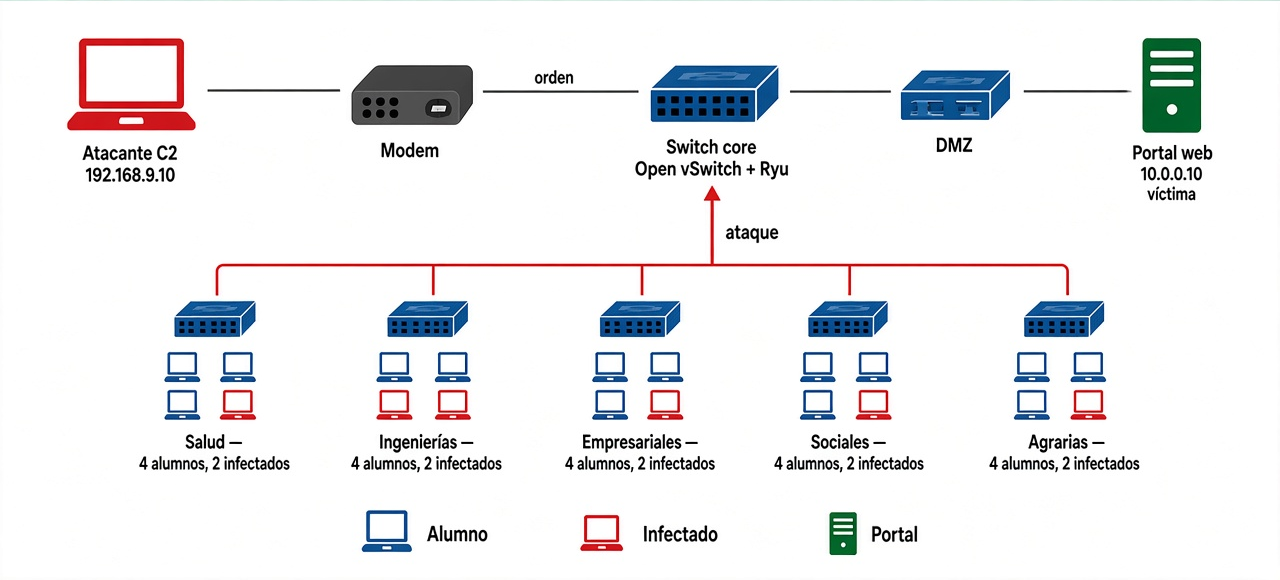
\includegraphics[width=\textwidth]{../MDPI/figures/topologia-campus-uncp.png}
\caption{Emulated topology. The C2 remains outside the campus;
compromised hosts attack the portal while students keep browsing.}
\label{fig:topologia}
\end{figure*}

\subsection{Software functionalities}
\texttt{scripts/docker/run\_scenario.sh} runs one scenario
(\texttt{baseline}, \texttt{synflood}, \texttt{httpflood},
\texttt{slowloris}, \texttt{icmpflood}) or all five; its
\texttt{repeat N} mode runs N independent repetitions, each with a
different seed and sampled attack intensities, so results can be
reported as mean~$\pm$~standard deviation instead of from a single run.
\texttt{scripts/mininet/flow\_monitor\_13.py} is the Ryu controller: it
learns like an L2 switch but installs IP-based flows and periodically
polls OpenFlow flow statistics, writing them per run.
\texttt{scripts/mininet/capture\_campus.py} stores the pcap and the
student probe. \texttt{scripts/mininet/pcap\_to\_csv.py} labels each
flow by source IP (a student stays \texttt{BENIGN} and a compromised
host takes the attack name) and merges the controller telemetry by
source IP. \texttt{scripts/mininet/build\_windows.py} builds a
time-window dataset (one row per second) from the portal counters and
the aggregated SDN telemetry.
\texttt{notebooks/analisis\_completo.py} trains the per-flow forest
without IP addresses and tests it on Ciencias Agrarias, while
\texttt{notebooks/deteccion\_ventanas.py} evaluates the per-window
detector with leave-one-run-out cross-validation and a feature-group
ablation.
\texttt{scripts/docker/preparar\_hibrido.sh} anonymizes authorized
student Wireshark captures, mixes them with simulation attacks, and
writes \texttt{notebooks/resultados/informe\_hibrido.txt}. The attack
is never run against the real campus network.

\subsection{Experimental design and variables}
Five independent scenarios are run: one baseline and four attacks.
Each lasts 120~s, starts from a clean topology and uses 20 students,
10 compromised hosts, one portal, one C2, one modem and seven
switches. The scenario is the independent variable. Responses are
HTTP availability, mean and 95th-percentile latency, packets per
second at the portal, maximum core flows, and container CPU, memory
and network use. The model receives bidirectional flow statistics
from CICFlowMeter and the ICMP aggregator.

\subsection{From pcap to the model}
The run in this article comes from one command,
\texttt{run\_scenario.sh all 120}. Inside the container, Open
vSwitch, Ryu and the topology start together. Each scenario lasts
120~s and leaves three artifacts: the pcap on the portal interface,
the student probe (HTTP status, latency, packets per second), and
container use sampled with \texttt{docker stats}.

\texttt{pcap\_to\_csv.py} splits each pcap in two. TCP and UDP go
through CICFlowMeter. ICMP is outside that filter, so a custom
aggregator closes a flow after 10~s. Without that cut, each
compromised host would leave one long flow and the class would
collapse to a handful of rows. The label does not come from the file
name. The JSON beside the pcap lists the compromised addresses. If
the source is one of those addresses and the scenario is not the
baseline, the flow takes the attack name. Students, the portal and
the whole baseline stay \texttt{BENIGN}. This run has 40{,}877 flows.
The baseline contributes 2{,}671, all benign. During an attack the
student flows stay inside the same CSV.

Before training, source IP, destination IP, both ports and the
timestamp are dropped. An infinity or a missing value becomes zero,
and any column that does not vary in the training set is removed. If
the IP stayed, the forest would memorize which machine is compromised
rather than how the flow behaves. The model is a forest of 200 trees
with class weights, because the SYN flood contributes 23{,}539 flows
and would otherwise dominate. The split is not random: Salud,
Ingenier\'ias, Empresariales and Sociales train it (32{,}784 flows)
and only Agrarias is tested (8{,}091).

\begin{figure*}[t]
\centering
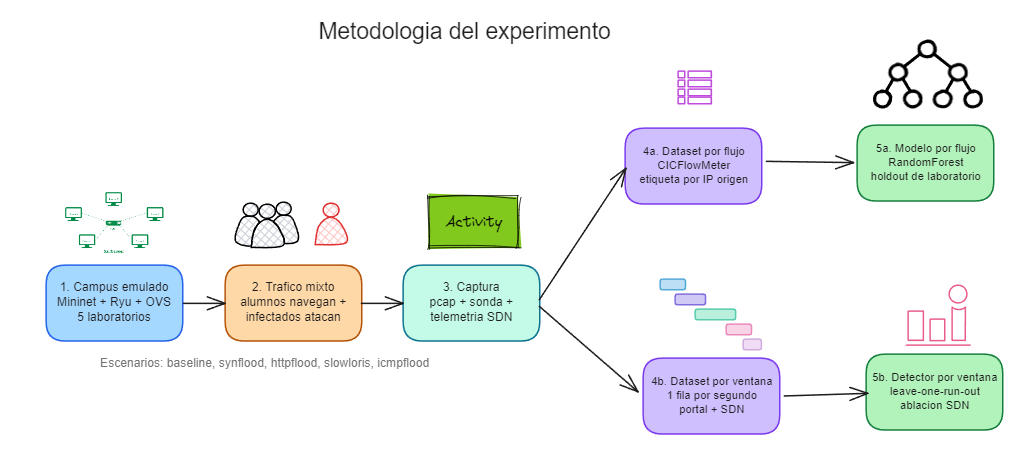
\includegraphics[width=\textwidth]{../MDPI/figures/metodologia-ddos-uncp.png}
\caption{Experimental pipeline from the emulated campus to the model.
The label comes from the sender, not the capture file.}
\label{fig:method}
\end{figure*}

\section{Results and impact overview}\label{sec:impact}
The single-vector reference dataset cannot be repeated, because its
benign traffic comes from the live internet
\citep{kumar2026icmpfloodsdn}. This testbed can be repeated, mixes
student and attack traffic in the same capture, and already yields a
classifier. On Ciencias Agrarias, a laboratory excluded from
training, macro F1 is \Fmacro. The probe states what the page feels,
not only which label was assigned. With institutional authorization,
the same pipeline admits real benign traffic (Wireshark) while keeping
the attack inside the container. The probe from that run is in
Table~\ref{tbl:sonda}: only Slowloris takes the portal down.

\subsection{Dataset composition}
The five CSVs contain 40{,}877 flows: 9{,}400 \texttt{BENIGN},
23{,}539 \texttt{synflood}, 7{,}188 \texttt{httpflood}, 630
\texttt{slowloris} and 120 \texttt{icmpflood}. This distribution
motivates class weighting and the decision not to claim ICMP as a
settled class. Fig.~\ref{fig:flows} also shows that attack captures
retain benign student flows.

\begin{figure}[t]
\centering
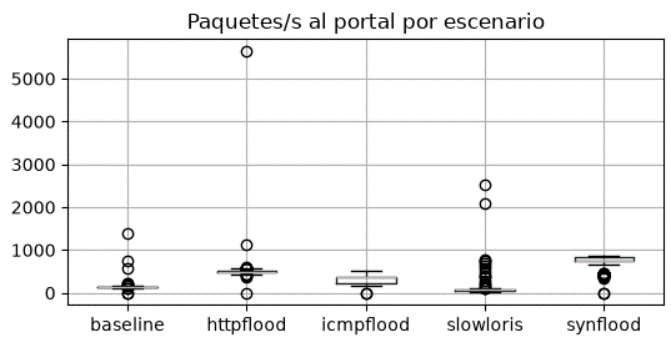
\includegraphics[width=\columnwidth]{../MDPI/figures/paquetes_escenario.png}
\caption{Benign and attack flows obtained in every scenario.}
\label{fig:flows}
\end{figure}

\subsection{Portal impact}
\begin{table}[t]
\centering
\small
\caption{Portal probe. Each scenario lasts 120~s.}
\label{tbl:sonda}
\setlength{\tabcolsep}{4pt}
\begin{tabular}{lrrrr}
\hline
Scenario & HTTP 200 & Failures & Latency (ms) & Packets/s \\
\hline
baseline & 120 & 0 & 407 & 111 \\
synflood & 120 & 0 & 404 & 466 \\
httpflood & 120 & 0 & 564 & 386 \\
slowloris & 1 & 117 & 403 & 86 \\
icmpflood & 120 & 0 & 404 & 271 \\
\hline
\end{tabular}
\end{table}


SYN produces the highest rate, 466 packets/s, yet the probe keeps 120
HTTP 200 responses. HTTP flood raises mean latency from 407 to
564~ms. Slowloris produces only 86 packets/s but occupies available
connections and fails 117 of 118 probes. Packet rate alone therefore
does not describe application impact.

\subsection{Classifier performance}
\begin{table}[t]
\centering
\small
\caption{Detection (random forest). Macro F1 \Fmacro.}
\label{tbl:deteccion}
\begin{tabular}{lrrrrp{2.6cm}}
\hline
Clase & Prec. & Recall & F1 & Flujos & On the flow \\
\hline
BENIGN & 0.956 & 0.949 & 0.953 & 1775 & well separated \\
httpflood & 0.939 & 0.947 & 0.943 & 1458 & well separated \\
icmpflood & 1.000 & 1.000 & 1.000 & 24 & too few flows to claim \\
slowloris & 1.000 & 1.000 & 1.000 & 126 & well separated \\
synflood & 1.000 & 1.000 & 1.000 & 4708 & well separated \\
\hline
\end{tabular}
\end{table}


Macro F1 on Agrarias is \Fmacro and binary benign-versus-attack F1 is
0.970. The most important features are forward average segment size,
forward packet-length mean and maximum, forward bytes and packet-size
variability. This is consistent with the scenarios: SYN repeatedly
sends small segments, HTTP exchanges complete requests and responses,
and Slowloris holds connections with little traffic.

\begin{figure}[t]
\centering
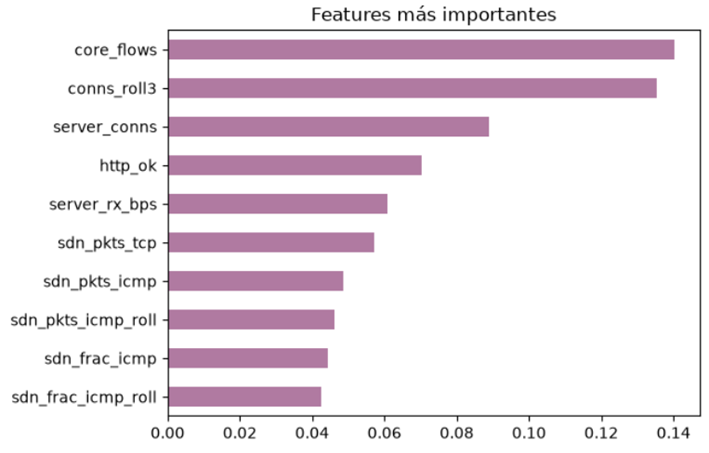
\includegraphics[width=\columnwidth]{../MDPI/figures/features_importantes.png}
\caption{Eight most important random-forest features.}
\label{fig:importance}
\end{figure}

\subsection{Testbed consumption}
Mean container CPU was 23\% for baseline, 26\% for SYN, 50\% for
HTTP, 523\% for Slowloris and 26\% for ICMP; in Docker, 100\%
corresponds approximately to one core. Slowloris occupied about five
of the six assigned cores, while observed peak memory remained below
200~MiB. These values cover the whole testbed, not only the victim.

\begin{figure}[t]
\centering
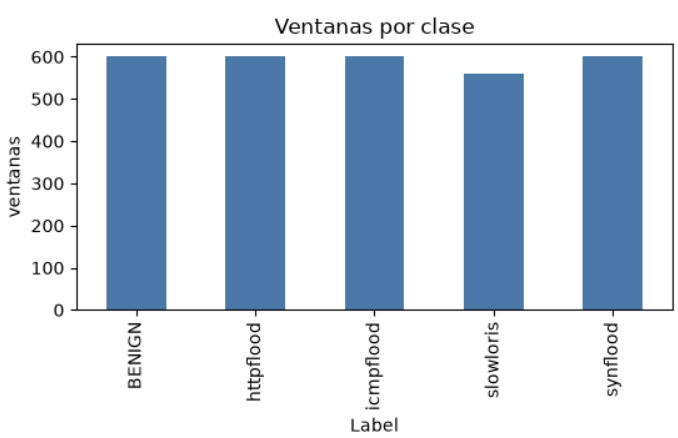
\includegraphics[width=\columnwidth]{../MDPI/figures/ventanas_por_clase.png}
\caption{Mean container CPU by scenario.}
\label{fig:cpu}
\end{figure}

\subsection{Discussion}
The home test supports the working hypothesis for four defensible
classes: macro F1 exceeds 0.90 without IP addresses and transfers to
a held-out laboratory. It does not demonstrate real-network
deployment or online detection. The contrast between SYN and
Slowloris also shows why flow classification should be paired with a
service probe: more packets do not necessarily mean lower service
availability.

\subsection{Ongoing research projects using the software}
The testbed is used in the authors' undergraduate thesis at the
Universidad Nacional del Centro del Per\'u. The Wireshark capture
protocol for the network officer is documented in
a separate document distributed with the software.

\subsection{Limitations and future improvements}
The table is still computed from emulated students. The hybrid
dataset (Wireshark plus simulated attack) is ready in the code and is
updated when the authorized pcaps arrive. The reported per-flow result
comes from a single 120~s run; the \texttt{repeat} driver and the
leave-one-run-out cross-validation now make the evaluation repeatable,
and the multi-run figures (mean~$\pm$~standard deviation) are being
regenerated. ICMP accounts for 120 flows in the whole set and 24
in the Agrarias test, so its perfect F1 is not reported as a settled
class result. The per-window detector is designed for early detection
and consumes the controller telemetry that a Ryu-side detector would
use, but it still scores already-captured windows offline rather than
running inside Ryu. Future work: report the multi-run cross-validated
figures and the SDN ablation, repeat the test with the Wireshark
background and a mixed four-vector scenario, add more ICMP samples, and
move the trained per-window model into the controller for online
detection.

\subsection{Conclusions}
The run already measured, taken at home inside Docker, is the base
of the proposal. In that run the student and the attack share the
capture, the model does not use IP addresses, and on Ciencias
Agrarias the macro F1 is \Fmacro. Sender-based labels preserve benign
traffic inside an attacked capture; a laboratory holdout is more
demanding than a random row split; and availability, packet rate and
classification describe different aspects of an incident. Only
Slowloris takes the portal down. ICMP is not claimed. This base
supports the request for authorized real benign traffic. The
simulated attack does not leave the container.

\subsection{List of scholarly publications enabled by this software}
There is no other publication yet. This software is what makes the
evaluation in this article possible.

\section{Software and hardware requirements}\label{sec:requirements}

The testbed runs in an Ubuntu 24.04 container. The versions in the
table were read inside the \texttt{ataque-sdn} image. The model was
trained with Python 3.12.3, scikit-learn 1.9.1 and pandas 3.0.6.
Ryu uses Python 3.9.25.

\begin{table}[t]
\footnotesize
\caption{Testbed setup requirements.}\label{tbl:testbed}
\begin{tabular}{@{}p{0.5cm}p{2.3cm}p{1.7cm}p{1.6cm}@{}}
\toprule
N.\textsuperscript{o} & Description & Tool & Version \\
\midrule
1 & Network emulator & Mininet & 2.3.0 \\
2 & Virtual switch & Open vSwitch & 3.3.9 \\
3 & SDN controller & Ryu & 4.34 \\
4 & SYN and ICMP flood & hping3 & 3.0.0-alpha-2 \\
5 & Low-rate attack & slowhttptest & 1.9.0 \\
6 & Packet capture & tcpdump & 4.99.4 \\
7 & pcap to CSV & CICFlowMeter & 0.5.0 \\
8 & Container OS & Ubuntu & 24.04 \\
\bottomrule
\end{tabular}
\end{table}

A conventional desktop is enough to repeat the run: 8 cores and
16~GB of RAM. Docker Desktop runs on Windows 11 or Ubuntu. The
container is given 6 CPUs and 8~GB, and Ubuntu 24.04 runs inside it.
Open vSwitch runs in userspace (\texttt{datapath netdev}).

\section*{Acknowledgements}
The authors thank the Universidad Nacional del Centro del Per\'u.

\bibliography{../MDPI/references}

\end{document}
